\documentclass[11pt, compress, tikz, xcolor=table]{beamer}
\usepackage{minted}
\usepackage{animate}

%%%%%%%%%%%%%%%%%%%%%%%%%%%%%%%%%% Styling for the beamer %%%%%%%%%%%%%%%%%%%%%%%%%%%%%%%%
%%%%%%%%%%%%%%%%%%%%%%%%%%%%%%%%%%%%%%%%%%%%%%%%%%%%%%%%%%%%%%%%%%%%%%%%%%%%%%%%%%%%%%%%%%

\setbeamertemplate{navigation symbols}{} 
\usetheme{Warsaw}

\setbeamertemplate{theorem begin}{{
\inserttheoremheadfont
\inserttheoremname
\inserttheorempunctuation
}}

\setbeamertemplate{theorem end}{}
\newtheorem{proposition}[theorem]{Proposition}

\theoremstyle{definition}
\newtheorem{mydef}[theorem]{Définition}
\makeatletter

\definecolor{beamer@blendedpurp}{rgb}{0.75, 0.2, 0.2}
  


\setbeamercolor{structure}{fg=beamer@blendedpurp}
\setbeamercolor*{palette quaternary}{fg=black,bg=white!80!gray }

\makeatother

\makeatletter
\defbeamertemplate*{footline}{shadow theme}
{%
  \leavevmode%
  \hbox{\begin{beamercolorbox}[wd=.5\paperwidth,ht=2.5ex,dp=1.125ex,leftskip=.3cm,rightskip=.3cm plus1fil]{title in head/foot}%
    \usebeamerfont{title in head/foot}\insertshorttitle%
  \end{beamercolorbox}}%
  \begin{beamercolorbox}[wd=.5\paperwidth,ht=2.5ex,dp=1.125ex,leftskip=.3cm plus1fil,rightskip=.3cm]{author in head/foot}%
    \usebeamerfont{author in head/foot}\hfill\insertframenumber\,/\,\inserttotalframenumber
  \end{beamercolorbox}%
  \vskip0pt%
}

\setbeamercolor*{section in toc}{fg=black}
\setbeamercolor*{enumerate item}{fg=black}
\setbeamercolor*{enumerate subitem}{fg=black}
\newcommand*{\rom}[1]{\expandafter\@slowromancap\romannumeral #1@}
\makeatother

%%%%%%%%%%%%%%%%%%%%%%%%%%%%%%%%%%%%%%%%%%%%%%%%%%%%%%%%%%%%%%%%%%%%%%%%%%%%%%%%%
%%%%%%%%%%%%%%%%%%%%%%%%%%%%%%%%%% end styling beamer %%%%%%%%%%%%%%%%%%%%%%%%%%%


\title{Covid Visualization}
\subtitle{Software development - HMMA238}
\author{Jihène Belgaied, Zakaria Laabsi, Chloé Serre-Combe and Stephani Ujka}
\date{\vspace*{-2cm}04/25/2021}
\institute[Montpellier University]{Student in Master of Statistics and Data Science at University of Montpellier}
\titlegraphic{%
  \makebox[0.9\paperwidth]{%
    \includegraphics[scale=.15]{images/logo_UM.png}%
    \hfill%
    
\includegraphics[scale=.05]{images/fds.png}%
    \hspace{.25cm}
  }%
}

\begin{document}

{
\def\mytitleframe{\bgroup
\makeatletter
\setbeamertemplate{footline}
{%
  \leavevmode%
  \hbox{\begin{beamercolorbox}[wd=.5\paperwidth,ht=2.5ex,dp=1.125ex,leftskip=.3cm,rightskip=.3cm plus1fil]{title in head/foot}%
    \usebeamerfont{title in head/foot}\insertshorttitle%
  \end{beamercolorbox}}%
  \begin{beamercolorbox}[wd=.5\paperwidth,ht=2.5ex,dp=1.125ex,leftskip=.3cm plus1fil,rightskip=.3cm]{author in head/foot}%
    \usebeamerfont{author in head/foot}%\hfill\insertframenumber\,/\,\inserttotalframenumber
  \end{beamercolorbox}%
  \vskip0pt%
}
\maketitle
\egroup
\addtocounter{framenumber}{-1}
}
\makeatother
	\mytitleframe
}



\begin{frame}
\frametitle{Table of contents}
  \tableofcontents
\end{frame}      
\setbeamertemplate{background}{}


\section{Introduction}

\begin{frame}[fragile]{Introduction}

The goal is to produce an animated map using covid data and to produce various charts linked to the analysis of the covid crisis. \newline

To this aim we create a covidviz module you can find here : \begin{center}\href{https://github.com/jihene-b3/covidviz}{\beamergotobutton{Github covidviz}}\end{center}\newline
\end{frame}


\section{Covidviz}
\subsection{Dependencies and import}
\begin{frame}[fragile]{Dependencies and import}

Package importation :
\begin{minted}{python}
>>> import covidviz as cvz
\end{minted}

\begin{block}{Specific dependencies}
\begin{enumerate}
\item $\texttt{pyDeck}$
\item $\texttt{ipywidget}$
\item $\texttt{folium}$
\item $\texttt{plotly}$
\item $\texttt{pandas\_alive}$
\item $\texttt{networkx}$
\item $\texttt{geopandas}$
\item $\texttt{dash}$

\end{enumerate}
\end{block}
\end{frame}

\subsection{Data}
\begin{frame}[fragile]{Data used}
\begin{center}
\begin{table}
\begin{tabular}{ccc}
\hline
\multicolumn{1}{l}{{\color[HTML]{000000} }} &
  \cellcolor[HTML]{C0C0C0}{\color[HTML]{000000} \textbf{Usage}} &
  \cellcolor[HTML]{C0C0C0}\textbf{Informations} \\ \hline
\cellcolor[HTML]{C0C0C0}{\color[HTML]{000000} \textbf{data.gouv.fr}} &
  \begin{tabular}[c]{@{}c@{}}animated maps\\ gif\\ stats\\ sparse matrix\\ graph\end{tabular} &
  \begin{tabular}[c]{@{}c@{}}covid deaths\\ covid hospitalized\\ patient transfers\\ intensive care unit (ICU)\\ screening\\ epidemio analysis\\ vaccine data\end{tabular} \\
  \hline
\cellcolor[HTML]{C0C0C0}{\color[HTML]{000000} \textbf{France GeoJSON}} &
  animated maps &
  \begin{tabular}[c]{@{}c@{}}geometry for \\ french departments \\ and regions\end{tabular} \\
  \hline
\cellcolor[HTML]{C0C0C0}{\color[HTML]{000000} \textbf{Santé Public France}} &
  statistics &
  age, gender \\ \hline
\end{tabular}
\end{table}
\end{center}

\end{frame}

\subsection{Module structure}
\begin{frame}[fragile]{Module structure}
        \centering
        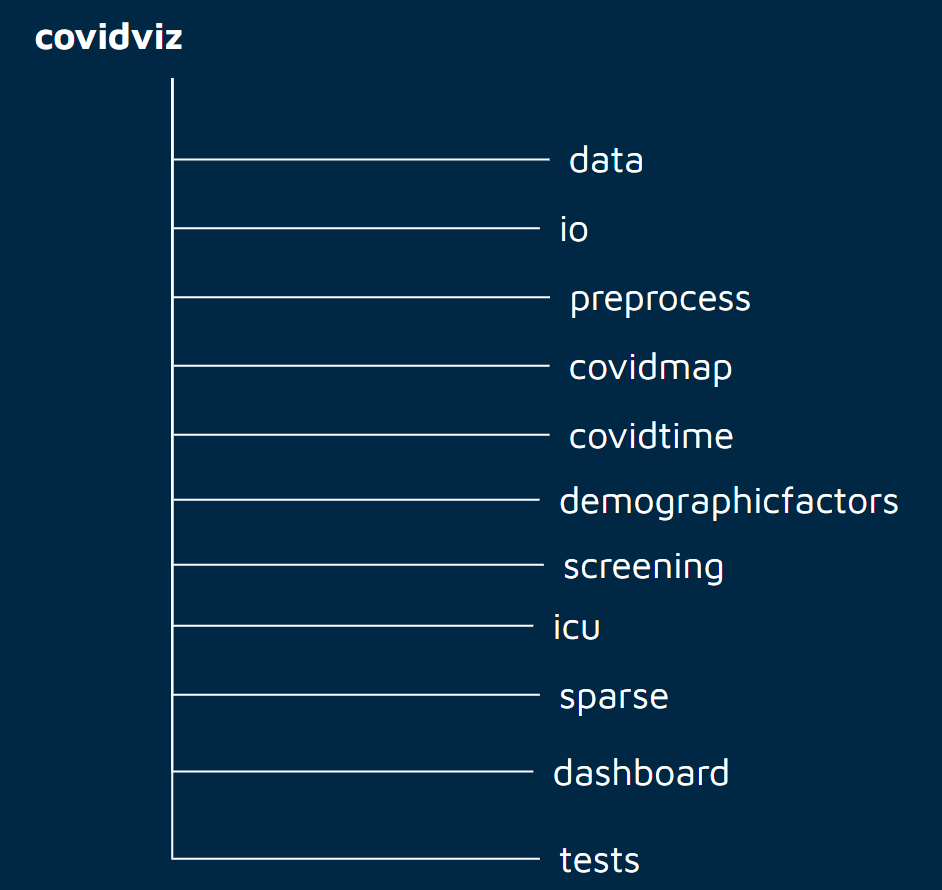
\includegraphics[scale=0.3]{images/structure.png}%

\end{frame}

\section{Animation}

\subsection{Animation Map}
\begin{frame}[fragile]{Animation Map}
\begin{columns}
          \column{0.38\linewidth}
             \centering
             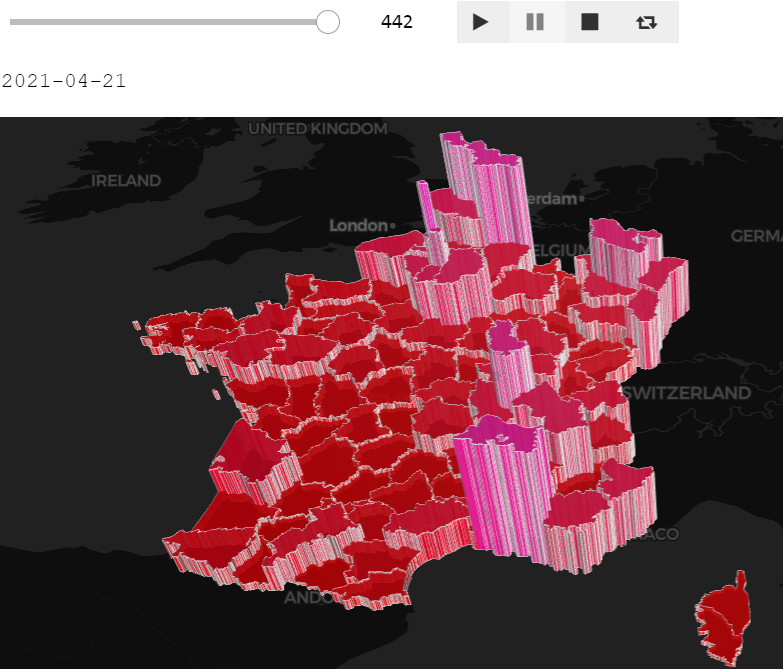
\includegraphics[height=5cm, width=5cm]{images/widget_map.png}
           \column{0.48\linewidth}
              \textbf{} \begin{enumerate}
                  \item Main code in $\texttt{covidviz/covidmap}$
                  \item A $\textt{Map\_covid}$ class
                  \item $\texttt{pyDeck}$ package
                  \item $\texttt{ipywidget}$ package
                  \item Parameters : \\
                    - departments or regions;\\
                    - deaths or hospitalized;\\
                    - time slider.\\
              \end{enumerate}
         \end{columns} 

\end{frame}

\begin{frame}[fragile]{Gif Animation} 

\paragraph{Main code in $\texttt{covidviz/covidtime}$.}\\

\paragraph{We used the $\texttt{pandas\_alive}$ package.}\\

\paragraph{The main function for generating gif visualizations is :}\\
 \begin{enumerate}
    \item $\texttt{covidtime/time\_gif/plot\_animation}$ with parameters :\\
        - regions or departments;\\
        - deaths or hospitalized.
    
\end{enumerate}

\end{frame}

\subsection{Gif animation}
\begin{frame}[fragile]{Gif animation}
             \centering
             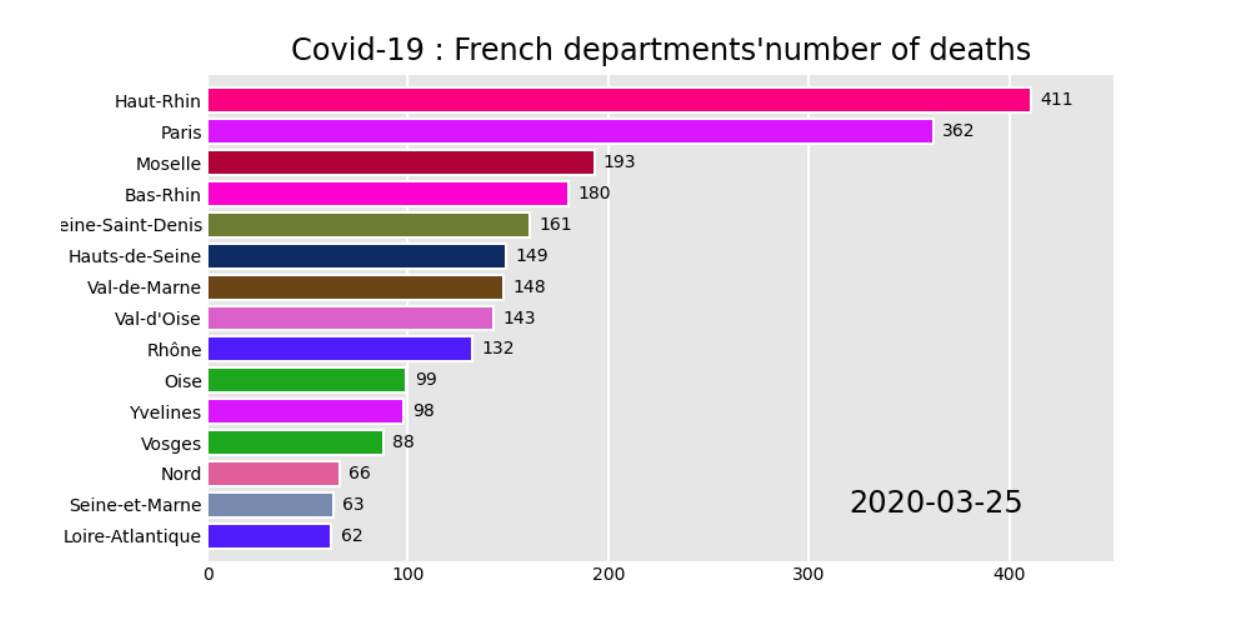
\includegraphics[height=8cm, width=11cm]{images/Capture_gif.PNG}
\end{frame}


\begin{frame}[fragile]{Covid Statistics} 

\paragraph{Main code in $\texttt{covidviz/demographicfactor}$.}\\

\paragraph{We used the $\texttt{plotly}$ package.}\\

\paragraph{One of the functions for generating charts is :}\\
 \begin{enumerate}
    \item $\texttt{demographicfactor/utils\_plot/df\_plot\_hosp}$
    \item $\texttt{parameters :}$\\
        - group age\\
        - date\\
        - number of people hospitalized\\
    \item $\texttt{time slider:}$\\

    
\end{enumerate}

\end{frame}

\section{Statistics}

\subsection{Covid Statistics}
\begin{frame}[fragile]{Covid Statistics}
      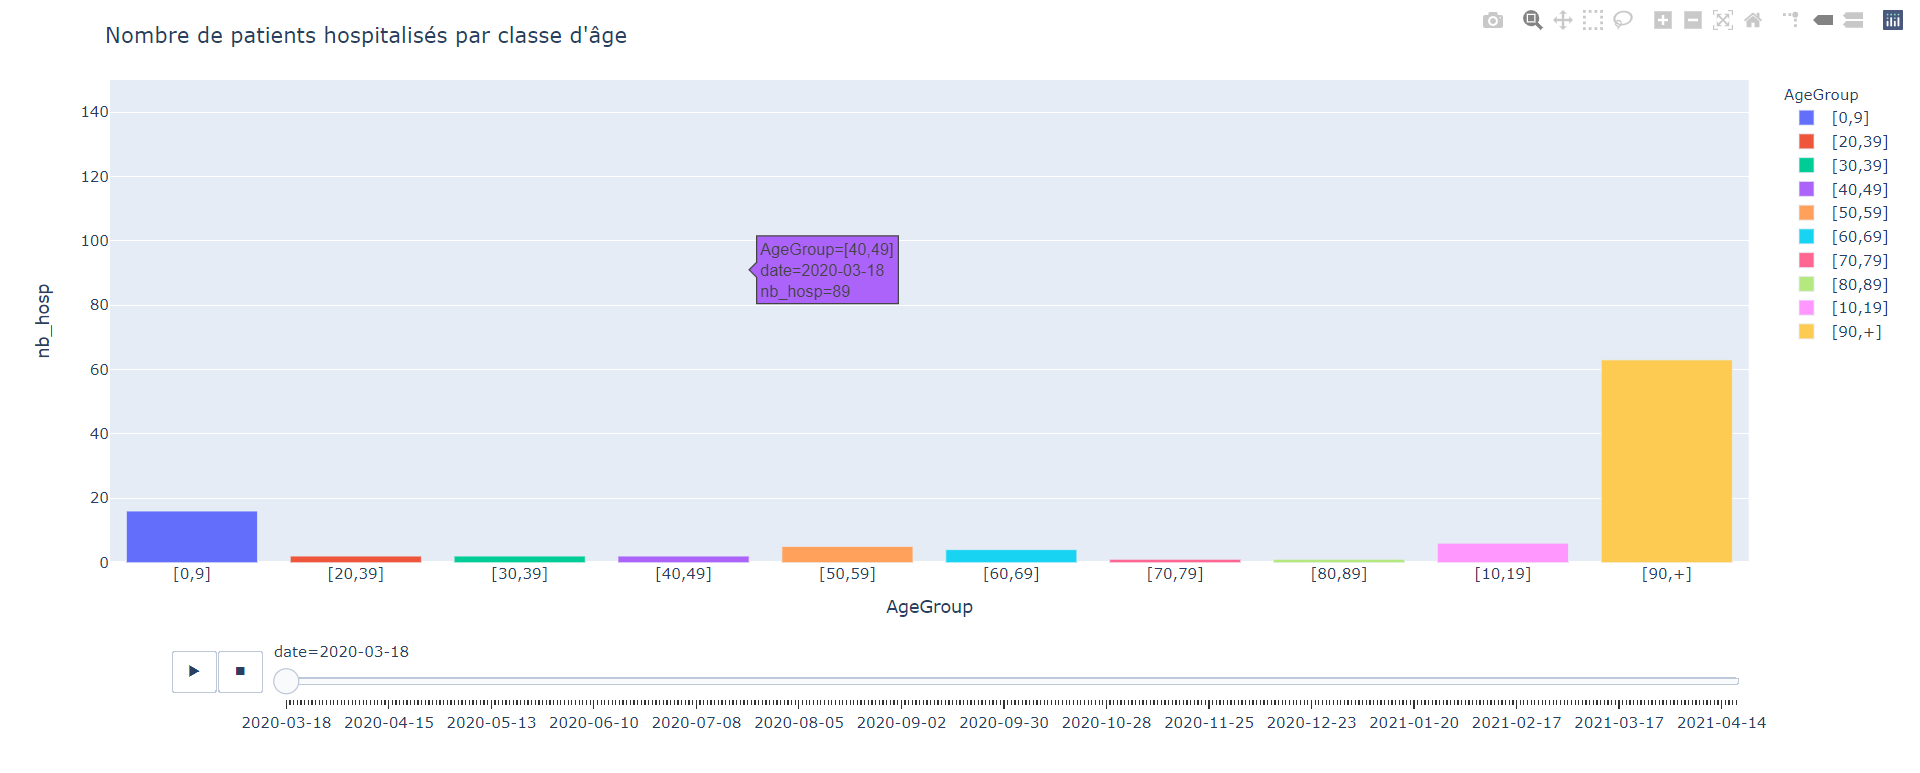
\includegraphics[width=11cm]{images/nombre_patient.PNG}
      
\end{frame}

\begin{frame}[fragile]{Covid Statistics} 

\paragraph{Main code in $\texttt{covidviz/covidtime}$.}\\

\paragraph{We used the $\texttt{matplotlib}$ package.}\\

\paragraph{The function used for generating the chart :}\\
 \begin{enumerate}
    \item $\texttt{covidtime/plot\_covidtracker/ratio}$
    \item $\texttt{parameters :}$\\
       -several lists for variables in df\_covid such us name locations ,number of hospitalizations;\\
       - current date.\\
    
\end{enumerate}

\end{frame}

\begin{frame}[fragile]{Covid Statistics}
      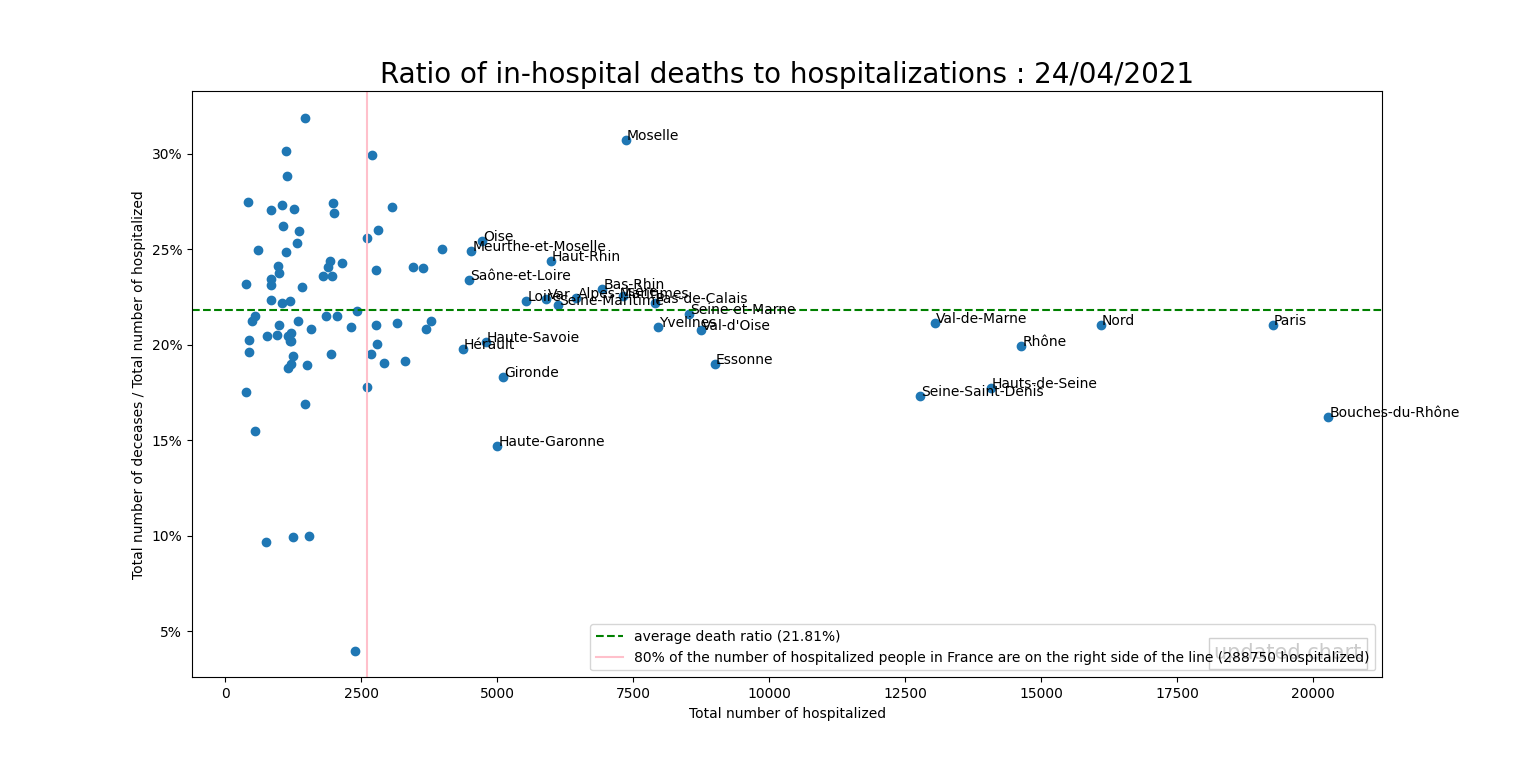
\includegraphics[width=12cm]{images/covidtracker.png}
      
\end{frame}



\subsection{ICU Statistics}
\begin{frame}[fragile]{ICU Statisics} 

\paragraph{Main code in $\texttt{covidviz/icu}$.}\\
\paragraph{We used the $\texttt{plotly}$ package.}\\
\paragraph{Some functions for many visualizations :}
 \begin{enumerate}
    \item $\texttt{icu\_dep\_display}$ with parameters : period, icu in each department.
    \item $\texttt{icu\_by\_reg\_display}$ with parameters : period, region, icu in each department of the region.
    \item $\texttt{icu\_all\_reg\_display}$
    with parameter : icu in each region.
    \item $\texttt{icu\_reg\_repartition}$
    with parameter : icu in each region.
    \item $\texttt{heat\_map\_icu\_reg}$ with parameter : icu in each region. 
 \end{enumerate}

\end{frame}


\begin{frame}[fragile]{ICU Statisics} 
       \centering
        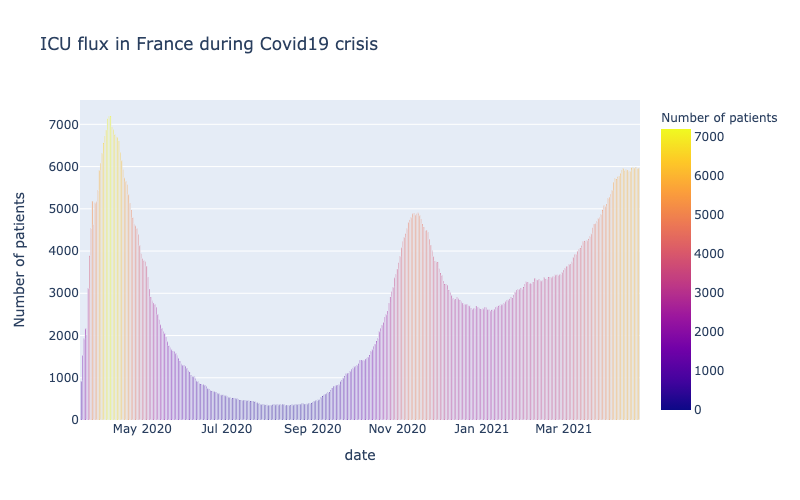
\includegraphics[width= 12 cm]{images/icu.png}\\

\end{frame}


\begin{frame}[fragile]{ICU Statisics} 
       \centering
        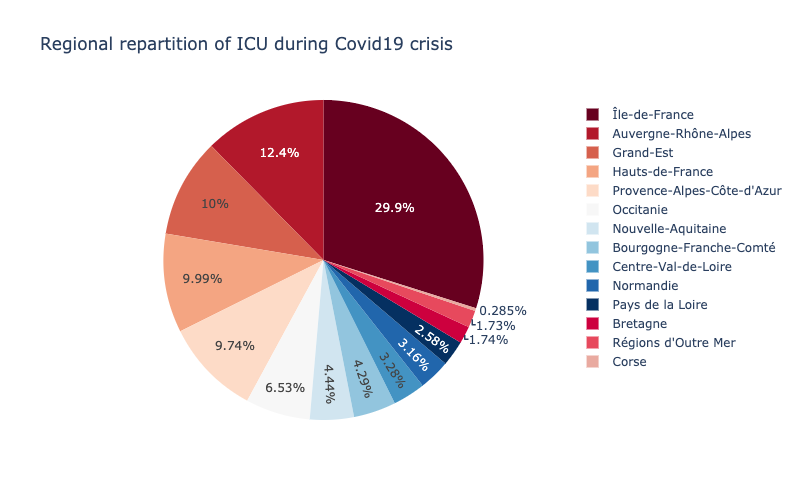
\includegraphics[width= 12 cm]{images/pie_chart.png}\\

\end{frame}


\subsection{Screening Statistics}
\begin{frame}[fragile]{Screening Statistics} 
\paragraph{Main code in $\texttt{covidviz/screening}$.}\\
\paragraph{We used $\texttt{plotly}$ and  $\texttt{folium}$ packages.}\\
\paragraph{Screening by different indicators :}
 \begin{enumerate}
    \item $\texttt{daily\_test}$ with parameters : department, classe age, tests performed.
    \item $\texttt{daily\_test\_dep}$ with parameters : department, tests performed.
    \item $\texttt{daily\_test\_age}$
    with parameter : classe age, tests performed.
 \end{enumerate}
 
 \paragraph{Maps of screening centers : $\texttt{map\_screening}$ function}
\end{frame}

\begin{frame}[fragile]{Screening Statistics} 
\begin{figure}
    \centering
    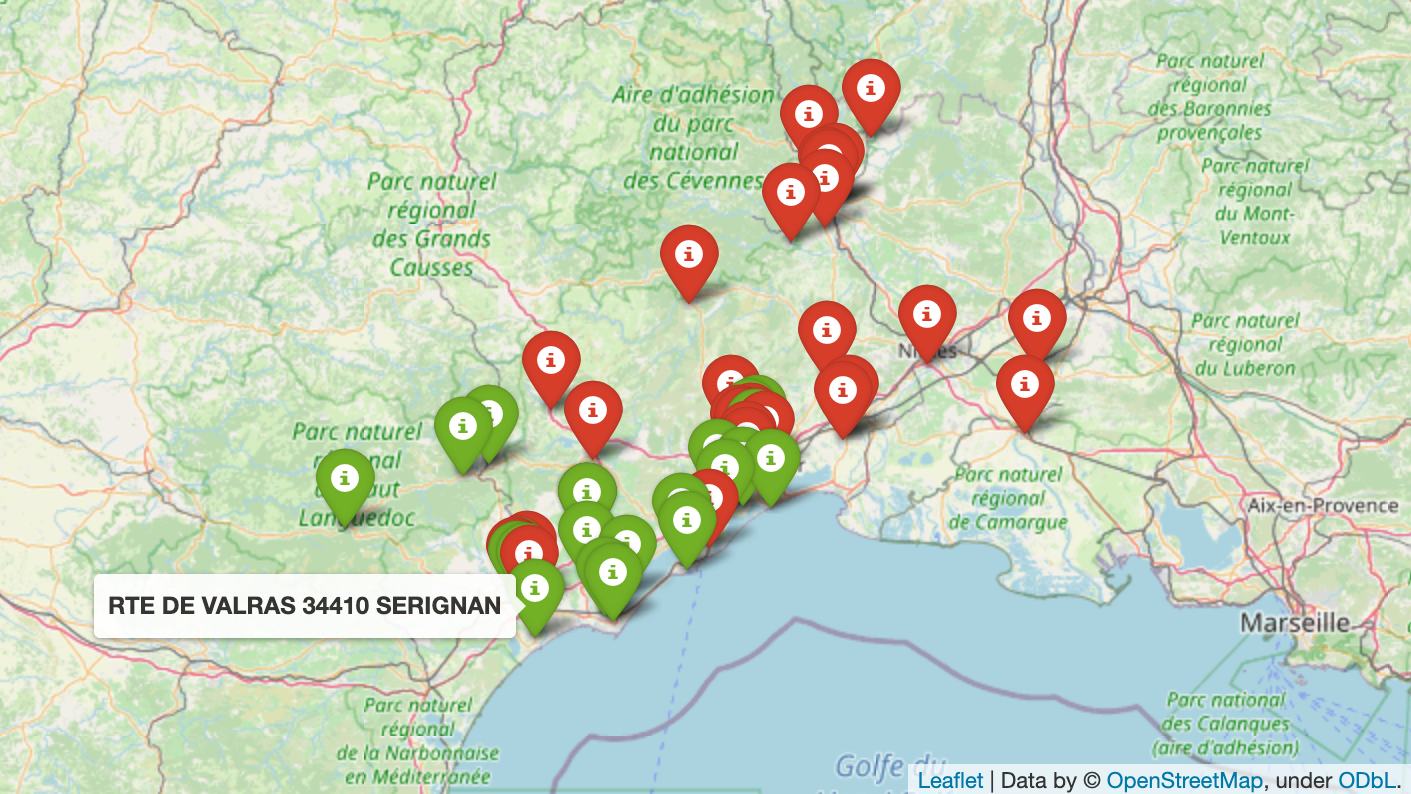
\includegraphics[width= 9 cm]{images/screening_map.png}
\end{figure}

\end{frame}

\section{Sparse}
\begin{frame}[fragile]{Sparse matrix and graph} 
    \begin{columns}
          \column{0.58\linewidth}
             \centering
             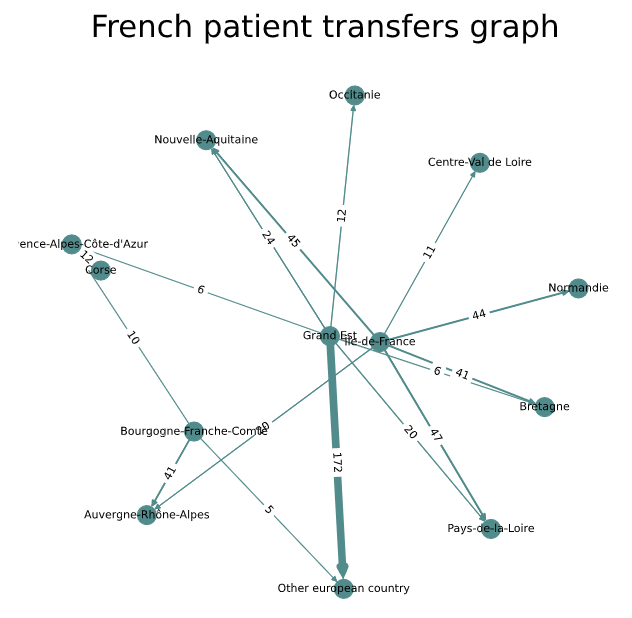
\includegraphics[height=7cm, width=7cm]{images/graph.png}
           \column{0.28\linewidth}
              \textbf{} \begin{enumerate}
                  \item Main code in $\texttt{covidviz/sparse}$
                  \item $\texttt{networkx}$ package
              \end{enumerate}
         \end{columns} 
\end{frame}


\section{Vaccine}

\subsection{Dashboard}
\begin{frame}[fragile]{Dashboard : Overview} 

\centering
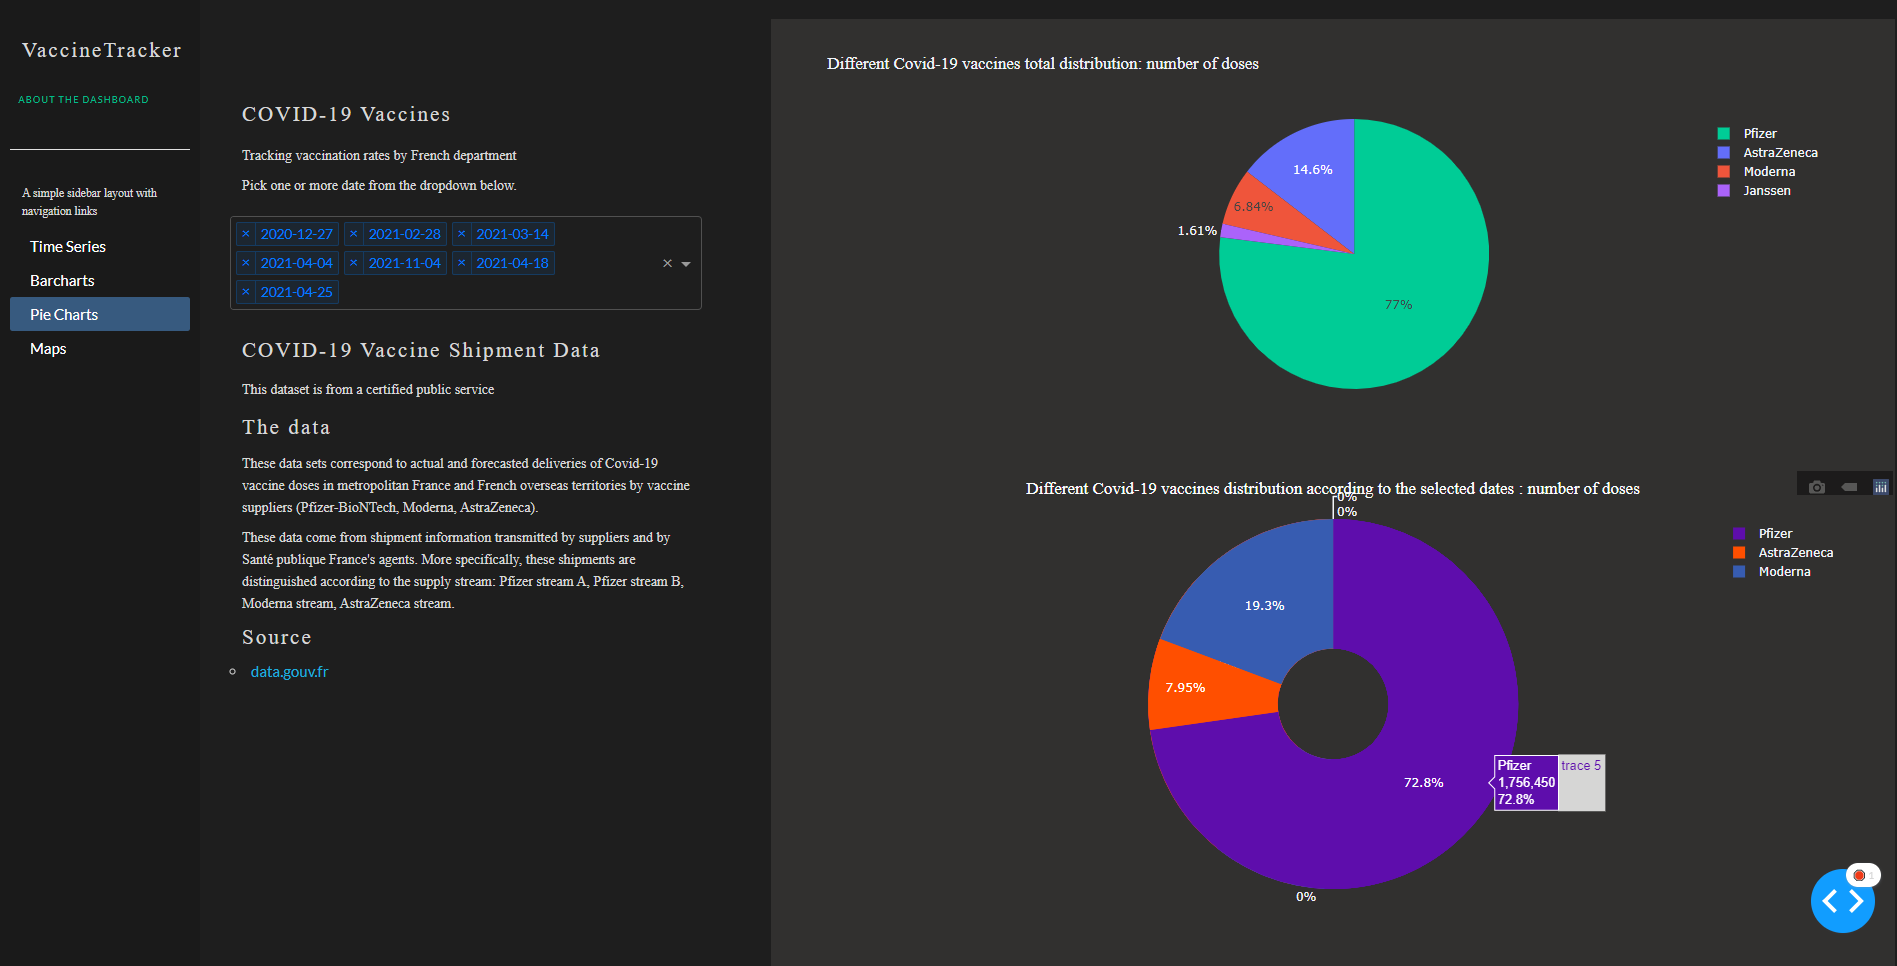
\includegraphics[width=\textwidth]{images/dashboard_sample.png}

\text{Dash app written in Python with the $\texttt{dash}$ package and $\texttt{Bootstrap}$ }\\
\text{Code available on \texttt{covidviz/dashboard}}

\end{frame}

\begin{frame}[fragile]{Dashboard : Callbacks} 

\centering
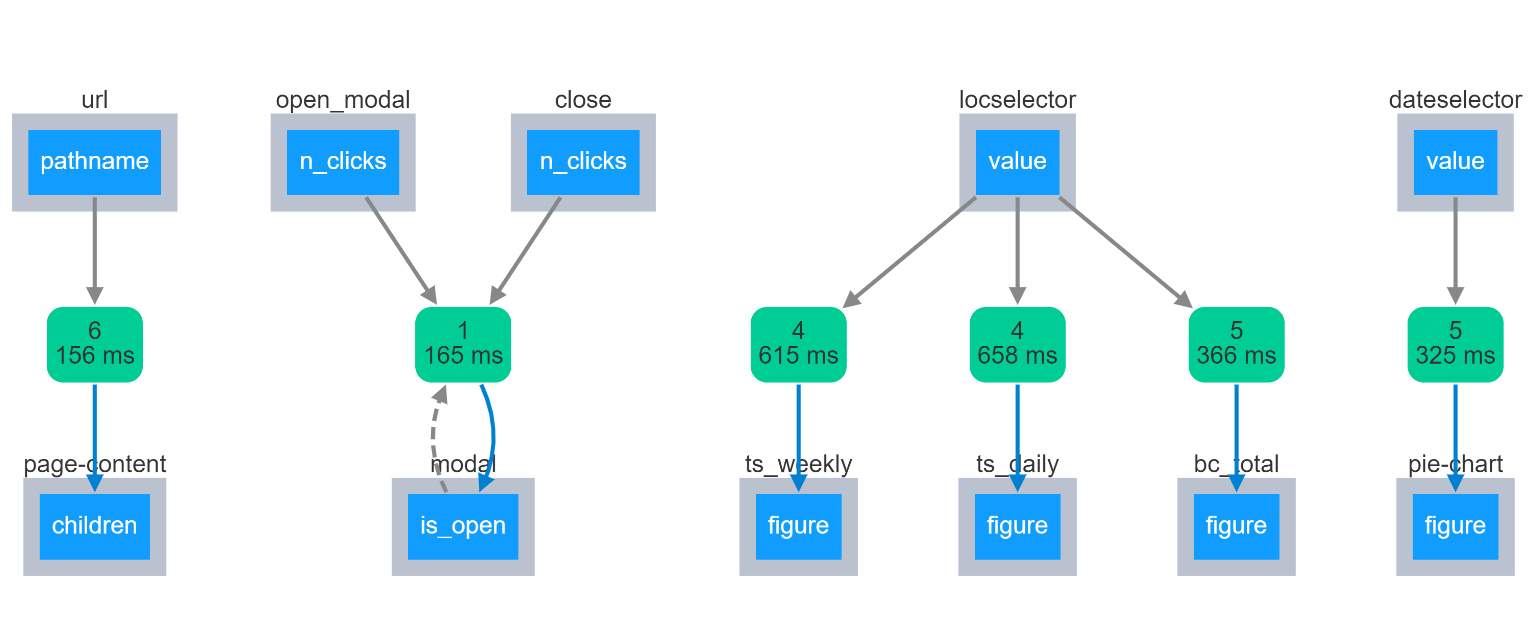
\includegraphics[width=\textwidth]{images/callbacks.png}

\text{Callbacks : adding interactivity.}\\
\textt{Inputs/Outputs are described as the arguments of the $\texttt{@app.callback}$ in the script}

\end{frame}

\begin{frame}[fragile]{Dashboard : Chart Example} 

\centering
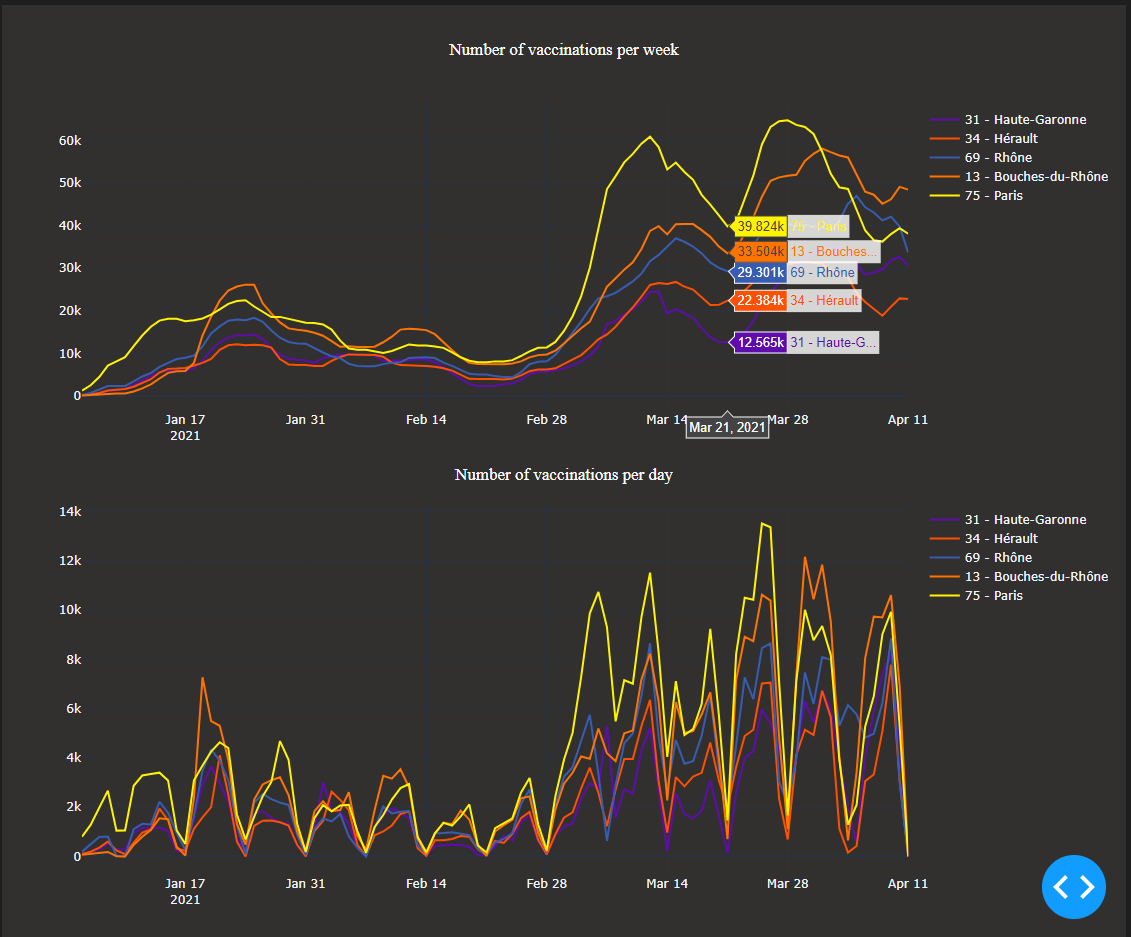
\includegraphics[width=\textwidth, height=6.5cm]{images/charts_dashboard.png}
\text{Time series made with the $\texttt{plotly}$ package. }\\
\text{Parameters: \textbf{number of vaccinations/ date/ departments}
}

\end{frame}

\begin{frame}[fragile]{Dashboard : 3D interactive map} 

\begin{columns}
          \column{0.58\linewidth}
             \centering
             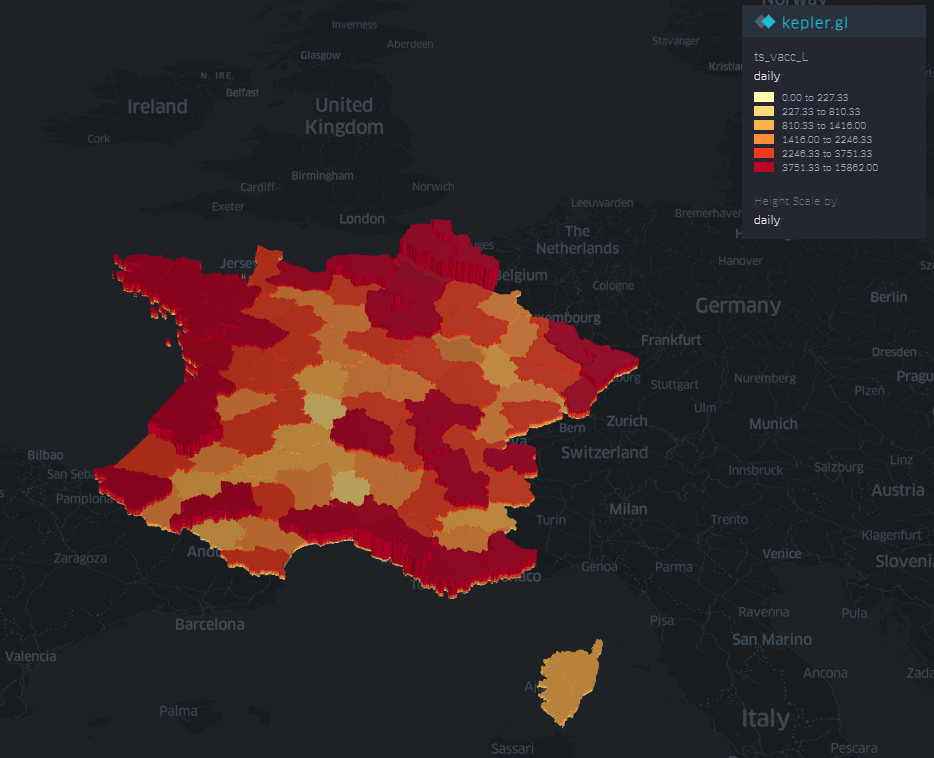
\includegraphics[height=7cm, width=7cm]{images/vacc_daily_map3D_kepler.png}
           \column{0.28\linewidth}
              \textbf{} \begin{enumerate}
                  \item Built with $\texttt{Kepler.gl}$ with $\texttt{MapGL}$ render
                  \item Time-series map
                  \item Display with the $\texttt{HTML}$ tag $\texttt{Iframe}$ in the dashboard
                  \item Available on $\texttt{/html files}$
              \end{enumerate}
         \end{columns} 

\end{frame}



\begin{frame}{Covid Visualization}
\centering
\textit{\textbf{Thank you}}\\
  For more information:  \href{https://github.com/jihene-b3/covidviz}{\beamergotobutton{Github covidviz}}
\end{frame}
\end{document}